\documentclass[11pt]{article}
%\documentclass{book}
\usepackage[utf8]{inputenc}
\usepackage[T1]{fontenc}
\usepackage[french]{babel}
\usepackage[top=1.8cm, bottom=1.8cm, left=1.8cm, right=1.8cm]{geometry}
\usepackage[linktocpage,colorlinks=false]{hyperref}
\usepackage{graphicx}
\usepackage{epsfig}
\usepackage{amssymb}
\usepackage{amsmath}
\usepackage{array}
\usepackage{subfig}
\usepackage{multicol}
\usepackage{caption}
\usepackage{listings}
\usepackage{algorithm}
\usepackage{algorithmic}
\hypersetup{
    colorlinks=true,
    breaklinks=true,
    urlcolor=red,
}
\parskip=5pt

\title{\huge{\textbf Spécifications}}
\author{AYOUB Pierre, BASKEVITCH Claire, BESSAC Tristan, \\
CAUMES Clément, DELAUNAY Damien, DOUDOUH Yassin}
\date{Mercredi 18 Avril 2018}

\begin{document}

\maketitle
\vspace{20em}
\begin{center}
\includegraphics{pictures/Application.png}\end{center}
\newpage

\tableofcontents

\newpage

\section{Introduction}

En réalisant le cahier des charges concernant l'application StegX, 
l'analyse des contraintes et des besoins du client nous amène à rédiger 
les spécifications. 

Le logiciel StegX pourra proposer de cacher des données dans des fichiers 
dont le format est pris en charge par l'application. De plus, un utilisateur 
pourra extraire les données cachées d'un fichier qu'on considère déjà comme 
hôte. StegX prendra en charge les trois algorithmes de stéganographie suivants : 
EOF, LSB et MetaData. 

Avec l'analyse des fonctionnalités de l'application, nous avons vu qu'elle 
devait gérer la manipulation de données binaires et donc il fallait un 
langage proche de la machine. 
De plus, nous devons implémenter des fonctions de stéganographie afin de 
cacher des données dans des fichiers. Par conséquent, une programmation 
procédurale était nécessaire. 
Enfin, il fallait des structures ou des objets simples afin de manipuler 
des structures de fichiers. 
De ce fait, nous avons choisi le langage C pour implémenter la future 
application StegX. En effet, le langage C propose une programmation procédurale, 
ainsi qu'un langage bas niveau proche de la machine. Enfin, la possibilité 
d'écriture et de lecture de bits et d'accès mémoire avec le langage C correspond 
à nos besoins. 
Sachant que StegX proposera une interface graphique, l'utilisation de GTK+ 
est possible en langage C. 
C'est donc pour toutes ces raisons que l'équipe de conception de StegX a 
choisi le langage C pour implémenter l'application. 

\section{Modules du produit}
\subsection{Organigramme}

\hspace{1cm}
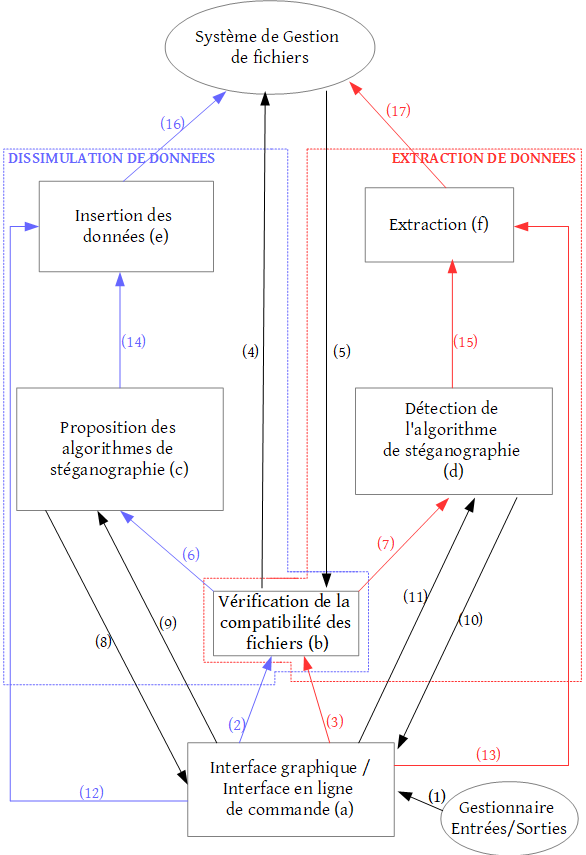
\includegraphics[scale=0.71]{pictures/organigramme.png}

\subsection{Liste des modules et de leurs fonctionnalités}

\begin{description}
\small
\item[a)] \textbf{Interface graphique / Interface en ligne de commande} :
    interfaces permettant à l'utilisateur de choisir parmi les deux
    fonctionnalités possibles de l'application. Il peut dissimuler des
    données dans un fichier (dont le type et le format sont pris en charge
    par l'application). Ou bien, il peut extraire les données cachées d'un
    fichier. \newline
    Il aura donc un mécanisme pour choisir le fichier hôte et le fichier 
    à cacher (pour la dissimulation de données), et un mécanisme pour choisir le 
    fichier contenant les données cachées à analyser (pour l'extraction de 
    données cachées). 
    

\item[b)] \textbf{Vérification de la compatibilité des fichiers} : le format 
	du fichier hôte (pour le module \textit{Dissimulation de données}) ou 
	le format du fichier à analyser (pour le module \textit{Extraction de données 
	cachées}), choisis par l'utilisateur, est vérifié pour savoir s'il est 
	bien pris en charge par l'application. \newline
	Il aura un mécanisme de lecture du fichier hôte : selon les formats 
	pris en charge, il y aura une batterie de tests pour déterminer le 
	format du fichier. 

\item[c)] \textbf{Proposition des algorithmes de stéganographie} : en fonction
    du type et du format du fichier hôte, ainsi que de la taille des données à
    cacher, un mécanisme proposera un ou plusieurs algorithmes (avec ou sans 
    sécurité supplémentaire). 

\item[d)] \textbf{Détection de l'algorithme de stéganographie} : un mécanisme 
	d'analyse du fichier permettra de découvrir quel algorithme a été utilisé 
	afin de les extraire correctement par la suite. 

\item[e)] \textbf{Insertion des données} : la copie des données du fichier hôte
    sera modifiée avec l'insertion des données à cacher à l'aide de l'algorithme
    choisi par l'utilisateur. 

\item[f)] \textbf{Extraction} : les données cachées dans le fichier à analyser
    sont extraites. Les algorithmes utilisés pour l'insertion des données 
    et l'extraction seront expliqués dans la sous-section \textit{"Algorithmes 
    de dissimulation et d'extraction en stéganographie"}

\end{description}

\subsection{Liste des informations qui circulent entre les modules}

\begin{multicols}{2}
\begin{description}
\footnotesize
\item[1)] 
\begin{itemize}
\item Utilisation de l'application (dissimulation ou extraction).
\item Nom du fichier hôte, nom du fichier à cacher et chemin du fichier à créer
    (pour la dissimulation).
\item Nom du fichier à analyser et chemin du fichier résultant de l'extraction
    des données cachées (pour l'extraction).
\end{itemize}
\item[2)] 
\begin{itemize}
\item Nom du fichier hôte.
\item Nom du fichier à cacher.
\end{itemize}
\item[3)] 
\begin{itemize}
\item Nom du fichier contenant les données cachées à analyser.
\end{itemize}
\item[4)] 
\begin{itemize}
\item Nom du fichier hôte et nom du fichier à cacher (pour la dissimulation).
\item Nom du fichier contenant les données cachées à analyser (pour
    l'extraction).
\end{itemize}
\item[5)]
\begin{itemize}
\item Fichier hôte et fichier à cacher (pour la dissimulation).
\item Fichier contenant les données cachées à analyser (pour l'extraction).
\end{itemize}
\item[6)]
\begin{itemize}
\item Fichier hôte.
\item Fichier à cacher.
\end{itemize}
\item[7)]
\begin{itemize}
\item Fichier contenant les données cachées à analyser.
\end{itemize}
\item[8)]
\begin{itemize}
\item Liste des algorithmes que l'utilisateur peut utiliser (selon le format du
    fichier hôte et la taille des données à cacher).
\end{itemize}
\item[9)]
\begin{itemize}
\item Choix de l'algorithme par l'utilisateur.
\item Mot de passe choisi par l'utilisateur (s'il a choisi l'option de protéger
    ses données par mot de passe).
\end{itemize}
\item[10)]
\begin{itemize}
\item Choix de l'algorithme détecté dans le fichier à analyser.
\end{itemize}
\item[11)]
\begin{itemize}
\item Mot de passe pour extraire les données (s'il a choisi l'option de
    protéger ses données par mot de passe).
\end{itemize}
\item[12)]
\begin{itemize}
\item Chemin du fichier à créer qui dissimulera les données à cacher et aura
    l'apparence du fichier hôte.
\end{itemize}
\item[13)]
\begin{itemize}
\item Chemin du fichier résultant de l'extraction des données cachées.
\end{itemize}
\item[14)]
\begin{itemize}
\item Fichier hôte.
\item Fichier à cacher.
\item Nom de l'algorithme de stéganographie utilisé.
\item Mot de passe choisi par l'utilisateur (s'il a choisi l'option de protéger
    ses données précédemment).
\end{itemize}
\item[15)]
\begin{itemize}
\item Fichier contenant les données cachées à analyser.
\item Nom de l'algorithme détecté.
\item Mot de passe choisi par l'utilisateur (s'il a choisi l'option de protéger
    ses données précédemment).
\end{itemize}
\item[16)]
\begin{itemize}
\item Données de l'hôte où les données à cacher ont été insérées en utilisant
    l'algorithme de stéganographie.
\end{itemize}
\item[17)]
\begin{itemize}
\item Données cachées extraites du fichier hôte.
\end{itemize}
\end{description}
  \ldots
\end{multicols}

\section{Description des structures et des types}

\section{Description des fonctions des différents modules}

\subsection{Module Interface graphique}
\subsection{Module Interface en ligne de commande}

\subsection{Module Vérification de la compatibilité des fichiers}

Ce module prend en entrée les chemins du fichier hôte et du fichier à 
cacher (pour la dissimulation) ; le chemin du fichier à analyser (pour 
l'extraction). Il va interagir avec le système de fichiers pour pouvoir 
vérifier la compatibilité des fichiers en entrée. 
Enfin, après sa vérification, ce module va envoyer les fichiers aux modules 
suivants. 
\newline

\begin{lstlisting}[language=c]
stegx_dissimulation stegx_check_compatibility_dissimulation 
                (char* host_name, char* hidden_name);
\end{lstlisting}

Cette fonction analyse la compatibilité des fichiers hôte et à cacher pour
la dissimulation. 
Pour cela, elle vérifie que les fichier hôte et à cacher existent et qu'ils 
ne sont pas vides. Ensuite, la fonction vérifie le format du fichier hôte. 
Elle va remplir les champs \textit{host}, \textit{hidden} et \textit{host\_type} 
de la structure \textit{stegx\_dissimulation} en entrée. 
\newline
\underline{Entrées :} \newline
\textit{host\_name :} chaine de caractères représentant le nom du fichier hôte. \newline
\textit{hidden\_name :} chaine de caractères représentant le nom du fichier à cacher. 
\newline
\underline{Sortie :} \newline
\textit{stegx\_dissimulation :} structure initialisée partiellement pour insérer les 
informations nécessaires à la vérification de la compatibilité des fichiers 
en entrée. 
\newline 

\begin{lstlisting}[language=c]
stegx_extraction stegx_check_compatibility_extraction (char* analysis_name);
\end{lstlisting}

Cette fonction analyse la compatibilité du fichier à analyser pour l'extraction. 
Pour cela, elle vérifie si le fichier à analyser existe et n'est pas vide. 
Ensuite, la fonction vérifie le format du fichier à analyser. 
Elle va remplir les champs \textit{analysis} et \textit{analysis\_type} 
de la structure \textit{stegx\_extraction} en entrée. 
\newline
\underline{Entrée :} \newline
\textit{analysis\_name :} chaine de caractères représentant le nom du fichier 
à analyser. \newline
\underline{Sortie :} \newline
\textit{stegx\_extraction :} structure initialisée partiellement pour insérer les 
informations nécessaires à la vérification de la compatibilité des fichiers 
en entrée. 
\newline 

\begin{lstlisting}[language=c]
int stegx_test_file_not_empty (stegx_file file);
\end{lstlisting}

Cette fonction teste si le fichier (représenté par la structure \textit{stegx\_file}
n'est pas vide. 
\newline
\underline{Entrée :} \newline
\textit{file :} structure représentant le fichier à tester. \newline
\underline{Sortie :} \newline
\textit{int :} renvoie 0 si le fichier est vide ou qu'il n'existe pas ; 1 sinon. 
\newline 

\begin{lstlisting}[language=c]
enum type stegx_test_file_bmp (stegx_file file);
enum type stegx_test_file_png (stegx_file file);
enum type stegx_test_file_wav (stegx_file file);
enum type stegx_test_file_mp3 (stegx_file file);
enum type stegx_test_file_avi (stegx_file file);
enum type stegx_test_file_flv (stegx_file file);
\end{lstlisting}

Ces fonctions testent le format du fichier en lisant le fichier en entrée 
(Magic Number notamment). 
\newline
\underline{Entrée :} \newline
\textit{file :} structure représentant le fichier à tester. \newline
\underline{Sortie :} \newline
\textit{int :} renvoie UNKNOWN si le format du fichier n'est pas pris en 
charge par l'application ; sinon, en fonction du format et des particularités 
du fichier, il peut renvoyer \textit{COMPRESSED\_BMP}, \textit{UNCOMPRESSED\_BMP}, 
\textit{PNG}, \textit{WAV\_PCM}, \textit{MP3}, \textit{COMPRESSED\_AVI}, 
\textit{UNCOMPRESSED\_AVI} ou \textit{FLV}. 
\newline 

\subsection{Module Proposition des algorithmes 
de stéganographie}
\subsection{Module Détection de l'algorithme de
stéganographie}
\subsection{Module Insertion des données}
\subsection{Module Extraction}

\section{Conclusion}


\end{document}
